\documentclass[11pt, oneside]{article}   	% use "amsart" instead of "article" for AMSLaTeX format
\usepackage{geometry}                		% See geometry.pdf to learn the layout options. There are lots.
\geometry{letterpaper}                   		% ... or a4paper or a5paper or ... 
%\geometry{landscape}                		% Activate for for rotated page geometry
%\usepackage[parfill]{parskip}    		% Activate to begin paragraphs with an empty line rather than an indent
\usepackage{graphicx}				% Use pdf, png, jpg, or eps� with pdflatex; use eps in DVI mode
								% TeX will automatically convert eps --> pdf in pdflatex		
\usepackage{amssymb}
\graphicspath{{/Users/telliott_admin/Dropbox/Tex/png/}}
\usepackage{parskip}

\title{Derivative of trigonometric functions}
%\author{The Author}
\date{}							% Activate to display a given date or no date

\begin{document}
\maketitle
%\section{}
%\subsection{}
\Large
The two most basic trigonometric derivatives are:
\[ \frac{d}{dx}\sin x = \cos x \]
\[ \frac{d}{dx}\cos x = -\sin x \]

\subsection*{sine}

The first of these comes from working with the difference quotient
\[ \lim_{h \rightarrow 0} \frac{\sin (x + h) - \sin x}{h} \]
using the sum formula for sine:
\[ \sin(x+h) = \sin x \cos h + \sin h \cos x \]
we obtain
\[ \lim_{h \rightarrow 0} \frac{\sin x \cos h + \sin h \cos x - \sin x}{h} \]
rearranging
\[ \lim_{h \rightarrow 0} \frac{\sin x( \cos h - 1)}{h} + \frac{\sin h \cos x}{h} \]
and since 
\[ \lim_{h \rightarrow 0} \frac{\sin h}{h} = 1 \]
the limit of the right-hand term  is $\cos x$.  On the other hand the limit of $\cos h - 1/h$ is $0$, so the left-hand term has a limit of $0$.

We've worked out these limits elsewhere.  The first one is quite famous, I'm sure you know it (or should know it).  The second can actually be derived from the first:

\[  \lim_{h \rightarrow 0}  \frac{\cos h - 1}{h} \times\frac{\cos h + 1}{\cos h + 1} \]
\[ =  \lim_{h \rightarrow 0}  \frac{\cos^2 h - 1}{h \cos h} \]
\[ =  \lim_{h \rightarrow 0}  \frac{- \sin h}{h}  \times \frac{\sin h}{\cos h} \]

The left-hand term is $-1$ (as above) and the right-hand term is $0/1 = 0$.

\subsection*{cosine}

The derivative of the cosine can also be obtained by using the difference quotient, but why don't we just try implicit differentiation plus the previous result:
\[ \sin^2 x + \cos^2 x = 1 \]
\[ \frac{d}{dx} (\sin^2 x + \cos^2 x) = 0 \]
\[ 2 \sin x \frac{d}{dx} \sin x + 2 \cos x \frac{d}{dx} \cos x = 0 \]
\[ 2 \sin x \cos x + 2 \cos x \frac{d}{dx} \cos x = 0 \]
\[ \sin x +  \frac{d}{dx} \cos x = 0 \]
You can see how this turns out!

\subsection*{tangent and secant}

What about other functions like $tan \ x$ and $sec \ x$?  We use the quotient rule.
\[ (\frac{u}{v})' = \frac{vu' - uv'}{v^2} \]
I check this mentally by considering $1/x$.  We pick up a minus sign from $-uv'$, which is what we want, so this is correct.
For $tan \ x$ we have:
\[ \frac{u}{v} = \frac{sin \ x}{cos \ x} \]
\[ (\frac{u}{v})' = \frac{cos^2x + sin^2x}{cos^2x} = \frac{1}{cos^2x} = sec^2x \]

Probably the most important of the rest is the secant, because of its connection with tangent (above)

\[  \frac{d}{dx} \frac{1}{\cos x} = \frac{- (-\sin x)}{\cos^2 x} \]
\[ = \sec \ x \tan \ x  \]

\subsection*{the rest of them}

We can use the quotient rule for these too, or we can just memorize them by their similarity with what we had already.

\[ \frac{d}{dx} \sec x =  \sec \ x \tan \ x  \]
\[ \frac{d}{dx} \csc x =  -\csc \ x \cot \ x  \]

and

\[ \frac{d}{dx} \tan x =  \sec^2 x  \]
\[ \frac{d}{dx} \cot x =  -\csc^2 x  \]

These are (perhaps) too hard to remember, but they are easy enough to derive with the quotient rule, and they will come in handy for evaluating various kinds of integrals.

\subsection*{inverse sine}

Suppose we label a right-triangle with sides $x$ (opposite the angle $y$) and $1$ for the hypotenuse.  Then

\[ \frac{x}{1} = \sin y \]
\[ y = \sin^{-1} x \]

$y$ is \emph{the angle whose sine is x}.  Where can we go from this?  Well, Pythagoras says that the adjacent side is $\sqrt{1-x^2}$, which is also $\cos y$.  What is the derivative of the inverse sine?  A trick is to start with the straightforward sine function:

\[ x = \sin y \]
\[ \frac{dx}{dy} = \cos y \]

but

\[ \cos y =  \sqrt{1-x^2} \]

Now, we want the derivative of the inverse sine, that is $dy/dx$:

\[ \frac{dy}{dx} = \frac{1}{\cos y} = \frac{1}{\sqrt{1-x^2}} \]

All this assumes that we limit the range of the inverse sine to the appropriate interval (domain:  $-1 \le x \le 1$;  range:  $-\pi / 2 \le y \le \pi/2$).

\begin{center} 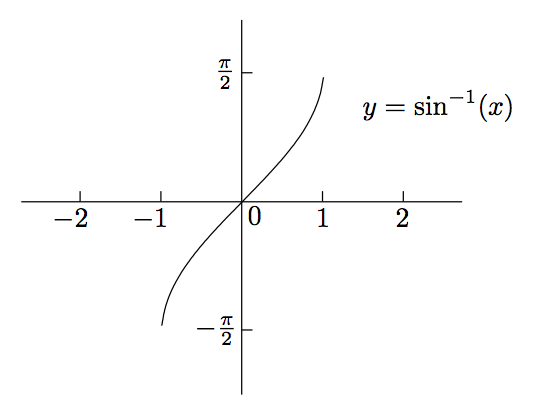
\includegraphics [scale=0.4] {arcsin.png} \end{center}

And above, we actually have to make a choice when we do $\sqrt{1-x^2}$.  We take the positive square root, and if you look at the figure, this is correct.  The function increases continuously, $f'(x)$ is positive on this interval.  (Except that it is not defined at the endpoints).

\subsection*{inverse cosine}

\begin{center} 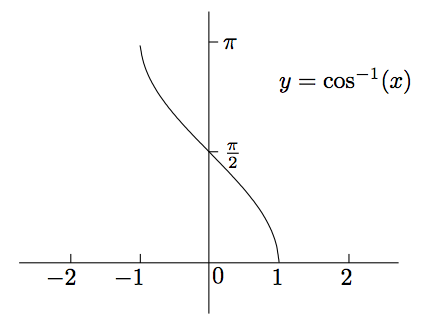
\includegraphics [scale=0.5] {arccos.png} \end{center}

As before, we limit the range of the inverse cosine to the appropriate interval (domain:  $-1 \le x \le 1$), however, the  range is different:  $0 \le y \le \pi$).  Also, if you look at the graph, the function is continuously decreasing over this interval (so we expect $f'(x)$ to be negative everywhere (except the endpoints, where it is not defined).

Now here is something curious:  if we plot them both together

\begin{center} 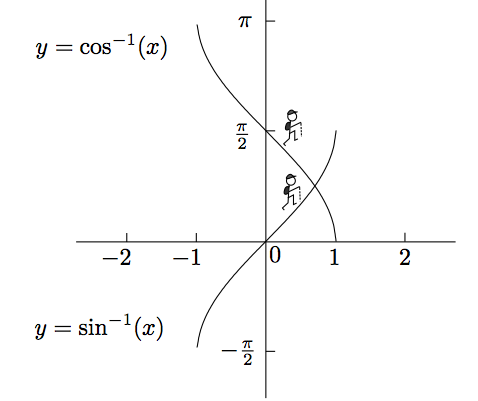
\includegraphics [scale=0.5] {arcsincos.png} \end{center}

Can you believe that if we add the two functions together, the result is a constant?  Actually

\[ \sin^{-1} x + \cos^{-1} x = \frac{\pi}{2} \]

Differentiating:

\[ \frac{d}{dx} \sin^{-1} x +  \frac{d}{dx} \cos^{-1} x = 0 \]

The derivative of inverse cosine is just the same as the derivative of the inverse sine, multiplied by $-1$!

\[ y = \cos^{-1} x \]
\[ \frac{dy}{dx} = - \frac{1}{\sqrt{1-x^2}} \]

If you want to see an actual calculation:

\[ y = \cos^{-1} x \]
\[ x = \cos y \]
\[ dx = -\sin y \ dy \]
\[ \frac{dy}{dx} = - \frac{1}{\sin y} = \]

Now, of course $x = \sin y$ but that doesn't really help us here.  Instead do this:

\[ \sin^2 y + \cos^2 y = 1 \]
\[ x = \cos y \]
\[ \sin^2 y + x^2 = 1 \]
\[ \sin y = \pm \sqrt{1-x^2} \]

so 

\[ y = \cos^{-1} x \]
\[ \frac{dy}{dx} = - \frac{1}{\sin y} = \pm \frac{1}{\sqrt{1-x^2}} \]

but remember that $f'(x) < 0$ everywhere so
\[ \frac{d}{dx} \cos^{-1} x = - \frac{1}{\sqrt{1-x^2}} \]

Let's go back to that curious statement about the sum of inverse sine and cosine:

\[ \sin^{-1} x + \cos^{-1} x = \frac{\pi}{4} \]

\begin{center} 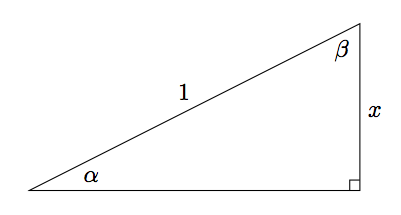
\includegraphics [scale=0.5] {sumarcsin.png} \end{center}

We'll call the angle $\alpha$ (originally $y$).  We have 

\[ \alpha = \sin^{-1} x \]
but 
\[ \beta = \cos^{-1} x \]
and 
\[ \alpha + \beta = \frac{\pi}{2} \]

Now, it's pretty easy to see how it works.

\subsection*{inverse tangent}

\begin{center} 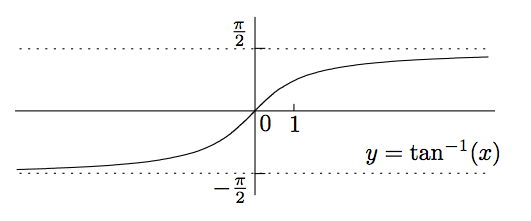
\includegraphics [scale=0.5] {arctan.png} \end{center}

Notice the domain and range, and that the slope is everywhere greater than $0$, except at the extrema.

\[ y = \tan^{-1} x \]
so 
\[ x = \tan y \]
\[ dx = \sec^2 y \ dy \]
We want
\[ \frac{dy}{dx} = \frac{1}{\sec^2 y}   \]
since 
\[ \sec^2 y = 1 + \tan^2 y \]
\[ \tan y = x \]
\[ \sec^2 y = 1 + x^2 \]
\[ \frac{d}{dx} \ \tan^{-1} x = = \frac{1}{\sec^2 y} = \frac{1}{1 + x^2}   \]

Remember the setup (this figure has the angle as $\alpha$ but we've gone back to using $y$).

\begin{center} 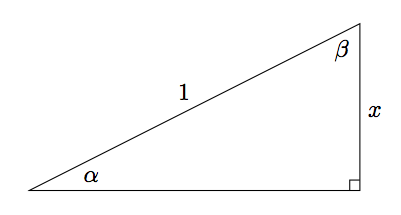
\includegraphics [scale=0.5] {sumarcsin.png} \end{center}

Why is this wrong?

\[ x = \sin y \]
\[ \sqrt{1 + x^2} = \cos y \]

So

\[ \frac{d}{dx} \tan^{-1} x= \cos^2 y  = 1 + x^2 \]




\end{document}  